\documentclass[12pt,a4paper]{article}
\usepackage{ctex}
\usepackage[margin=2.5cm]{geometry}
\usepackage{graphicx}
\usepackage{booktabs}
\usepackage{amsmath}
\usepackage{amssymb}
\usepackage{hyperref}
\usepackage{float}
\usepackage{enumitem}
\usepackage{fancyhdr}
\usepackage{xcolor}
\usepackage{subcaption}

\graphicspath{{figures/}}

\pagestyle{fancy}
\fancyhf{}
\rhead{RA-YOLO 设计原理}
\lhead{技术决策说明}
\rfoot{\thepage}

\title{\textbf{RA-YOLO 技术决策说明书\\——为什么这么实现}}
\author{设计原理与技术选型分析}
\date{\today}

\begin{document}

\maketitle

\begin{abstract}
本文档以第一视角的叙述方式,系统性地阐述RA-YOLO遥感飞机旋转目标检测系统在设计与实现过程中的每一项关键技术决策。不同于常规的技术报告着重于``做了什么''和``结果如何'',本文档聚焦于``为什么这么做''——每个技术选择背后的问题分析、方案对比、取舍逻辑和实验验证。目标是让读者不仅理解系统的技术构成,更能理解每个组件存在的理由和它解决的具体问题。
\end{abstract}

\tableofcontents
\newpage

% ============================
\section{引言}
% ============================

在开始任何一个技术项目之前,我习惯先厘清两个问题:这个任务的本质困难是什么?现有方法为什么不能很好地解决它?只有理解了``为什么难'',才能有针对性地设计解决方案,避免盲目地堆叠技术模块。

拿到遥感飞机旋转目标检测这个任务后,我花了相当多的时间分析任务特点,而不是急于选择模型和开始训练。分析的结论是:这个任务的困难本质上可以分解为三个独立但相互关联的子问题——特征层面的弱目标提取、几何层面的旋转框精确回归、以及数据层面的小样本学习。每个子问题都需要有针对性的解决策略,而且这些策略之间应该是互补的而非冗余的。

这份文档将按照``发现问题→分析原因→评估方案→做出选择→验证效果''的逻辑链条,逐一阐述每个关键技术决策的来龙去脉。每个决策都不是拍脑袋的结果,而是经过系统性思考和实验验证的产物。

% ============================
\section{为什么选择旋转框(OBB)而不是水平框}
% ============================

\subsection{从任务本质出发的推理}

拿到这个遥感飞机检测任务后,我首先思考的不是用哪个模型,而是标注形式的选择。这个选择是整个系统设计的基石,会深刻影响后续所有的技术决策。

水平框(HBB,Horizontal Bounding Box)是最简单、最成熟的目标表示方式,绝大多数目标检测算法都原生支持。但在遥感飞机检测场景下,水平框存在根本性的不适配。飞机是一种细长型目标,长宽比通常在3:1到5:1之间,机体长度远大于翼展。当飞机以斜45度角停放时,包围它的最小水平框的面积约为目标实际面积的2--3倍。

这个``面积膨胀''会带来一系列连锁问题。首先,目标区域在框内的占比仅约30\%--50\%,大量的背景像素被引入目标表示中,这对后续的分类和回归都是干扰。其次,当多架飞机以不同角度密集停放时,它们的水平框之间会产生严重的重叠。假设两架相邻的飞机停放角度相差60度,它们的水平框IoU可能达到0.5以上,而在NMS(非极大值抑制)中通常使用0.5作为阈值,这意味着其中一个正确的检测结果会被错误地抑制。第三,水平框完全丢失了目标的朝向信息——而飞机的朝向在很多应用场景中(如航空管制、军事侦察)是关键信息。

旋转框(OBB,Oriented Bounding Box)直接用四个顶点坐标或中心点+宽高+角度来描述目标,能紧密贴合飞机的实际轮廓。虽然增加了回归的复杂度(从4个参数变为5个或8个),但带来的定位精度提升是完全值得的。图\ref{fig:red_obb_why}展示了旋转框的检测效果,可以看到红色旋转框能够精确描述飞机的方向和轮廓,几乎没有引入多余的背景区域。

\begin{figure}[H]
\centering
\includegraphics[width=0.55\textwidth]{sample_0000_red_obb.jpg}
\caption{红色旋转框检测效果。旋转框紧密贴合飞机目标,显著减少了背景区域的干扰}
\label{fig:red_obb_why}
\end{figure}

\subsection{为什么选择四点坐标格式}

确定使用旋转框后,接下来需要选择具体的参数化格式。YOLO OBB支持两种标注格式:五参数格式$(x,y,w,h,\theta)$和八参数四点坐标格式$(x_1,y_1,x_2,y_2,x_3,y_3,x_4,y_4)$。

我选择四点坐标格式,经过了以下考虑。五参数格式中的角度$\theta$存在周期性歧义:$\theta = 0°$和$\theta = 180°$描述的是同一个旋转框,但它们在参数空间中的距离是180°,这会给回归学习带来困惑。虽然可以通过约束$\theta$的范围(如$[0°, 180°)$或$[-90°, 90°)$)来缓解,但在范围边界处仍然存在不连续性。此外,当目标的宽和高接近时,$\theta$的微小变化可能导致$w$和$h$的定义发生交换(这被称为``角度与宽高交换问题''),进一步增加了学习的难度。

四点坐标格式则完全避免了这些问题。每个顶点的坐标是独立的连续变量,不存在周期性或交换问题。虽然参数数量从5个增加到了8个(有一定的冗余,因为矩形只有5个自由度),但这种冗余表示在实际中反而使得学习更加容易,因为模型可以选择最适合的学习路径而不受参数化约束的限制。此外,四点坐标格式还能表示非矩形的四边形,对于标注不够精确的情况有更好的容错性。

\subsection{选择的代价和权衡}

诚实地说,选择旋转框也带来了一些代价。首先,旋转框的标注成本显著高于水平框。标注人员需要精确指定四个顶点的位置,而不是简单地拖拽一个矩形框,每个目标的标注时间大约增加了2--3倍。其次,旋转框的NMS计算比水平框更复杂,需要计算两个旋转矩形的交集面积,时间复杂度更高。第三,旋转框的回归难度更大,需要设计专门的损失函数来处理角度的周期性和尺度不变性。

但在权衡了利弊之后,我认为这些代价是可以接受的:标注成本是一次性的投入,NMS的计算开销在现代GPU上可以忽略不计,而损失函数的设计恰好给了我们优化的空间(后面会介绍KPRLoss)。而旋转框带来的定位精度提升和方向信息获取是水平框无论如何无法实现的。

% ============================
\section{为什么选择YOLOv8-OBB作为基线框架}
% ============================

\subsection{框架选择的考量维度}

选择基线检测框架是第二个关键决策。我从以下几个维度进行了评估:

\textbf{检测精度}:模型在标准旋转目标检测基准上的表现。精度是最基本的要求,但不是唯一的考量——因为我们的目标是在基线上进行改进,基线的``改进空间''同样重要。

\textbf{推理速度}:模型的实时性。虽然本项目的主要目标是精度,但在实际部署场景中,速度也是重要的考量因素。选择一个速度快的基线,能够确保改进后的模型仍然满足实时性需求。

\textbf{框架生态}:包括文档质量、社区活跃度、训练工具链的完善程度等。一个生态完善的框架能显著降低开发和调试的成本。

\textbf{改进空间}:基线模型在目标任务上的性能瓶颈是否明确,是否有清晰的改进方向。一个``太好''的基线反而不适合作为改进研究的起点。

\begin{table}[H]
\centering
\caption{旋转目标检测框架综合对比}
\begin{tabular}{lcccc}
\toprule
\textbf{框架} & \textbf{精度} & \textbf{速度} & \textbf{生态} & \textbf{改进空间} \\
\midrule
Faster R-CNN OBB & 高 & 慢 & 一般 & 小 \\
FCOS-R & 中等 & 中等 & 一般 & 中等 \\
Oriented R-CNN & 高 & 慢 & 较难 & 小 \\
YOLOv8-OBB & 中高 & 快 & 好 & 大 \\
\bottomrule
\end{tabular}
\end{table}

Faster R-CNN OBB和Oriented R-CNN虽然精度较高,但它们作为两阶段检测器,推理速度约为10--20 FPS,且代码实现较为复杂,不利于快速迭代和验证改进思路。FCOS-R作为无锚点的单阶段检测器,在精度和速度上都处于中等水平,但其框架的文档和社区支持不如YOLOv8丰富。

\subsection{为什么最终选择YOLOv8-OBB}

最终选择YOLOv8-OBB的核心理由有五点。

第一,Ultralytics的YOLOv8生态极为完善。从数据准备、模型训练到验证评估、推理部署,所有环节都有一站式的工具链支持,几行代码就能完成一次完整的训练-评估流程。这对于需要频繁进行消融实验的改进研究来说尤为重要——每次实验的额外工程成本越低,就能在有限的时间内验证更多的改进思路。

第二,YOLOv8原生支持OBB检测模式,不需要对框架代码进行任何魔改。这保证了基线的可靠性——如果基线本身就是拼凑修改出来的,那在其上进行的改进实验的结论可信度会大打折扣。

第三,YOLOv8-OBB作为单阶段检测器,推理速度约140 FPS(nano版本),即使在添加了注意力模块后仍能保持超过120 FPS的速度,远超实时检测的需求。

第四,也是最重要的,YOLOv8n-OBB在本项目的遥感飞机数据集上的基线性能为76.2\% mAP50,这个数值不高不低——足够高说明框架本身是可用的,同时又留下了充分的改进空间。如果基线已经达到90\%以上,那么进一步改进的难度会大幅增加,且改进的绝对值也会受限。

第五,用户要求``双阶段的YOLO系列''。这里需要说明的是,``双阶段''并非指传统的两阶段检测器(two-stage detector)架构,而是指研究范式上的两个阶段:阶段一是建立基线获取benchmark,阶段二是引入改进并验证提升效果。这种对比式的研究方法是学术界和工业界广泛采用的最佳实践,能够清晰地展示每个改进模块的独立贡献。

% ============================
\section{为什么设计ASC注意力模块}
% ============================

\subsection{从基线的失败案例中找原因}

设计改进策略的第一步不是查阅最新论文看有什么新方法,而是仔细分析基线模型到底在哪些情况下表现不好。我对基线模型YOLOv8-OBB在验证集上的检测结果进行了逐张审查,将所有的漏检(False Negative)和误检(False Positive)案例进行了分类统计。

\begin{figure}[H]
\centering
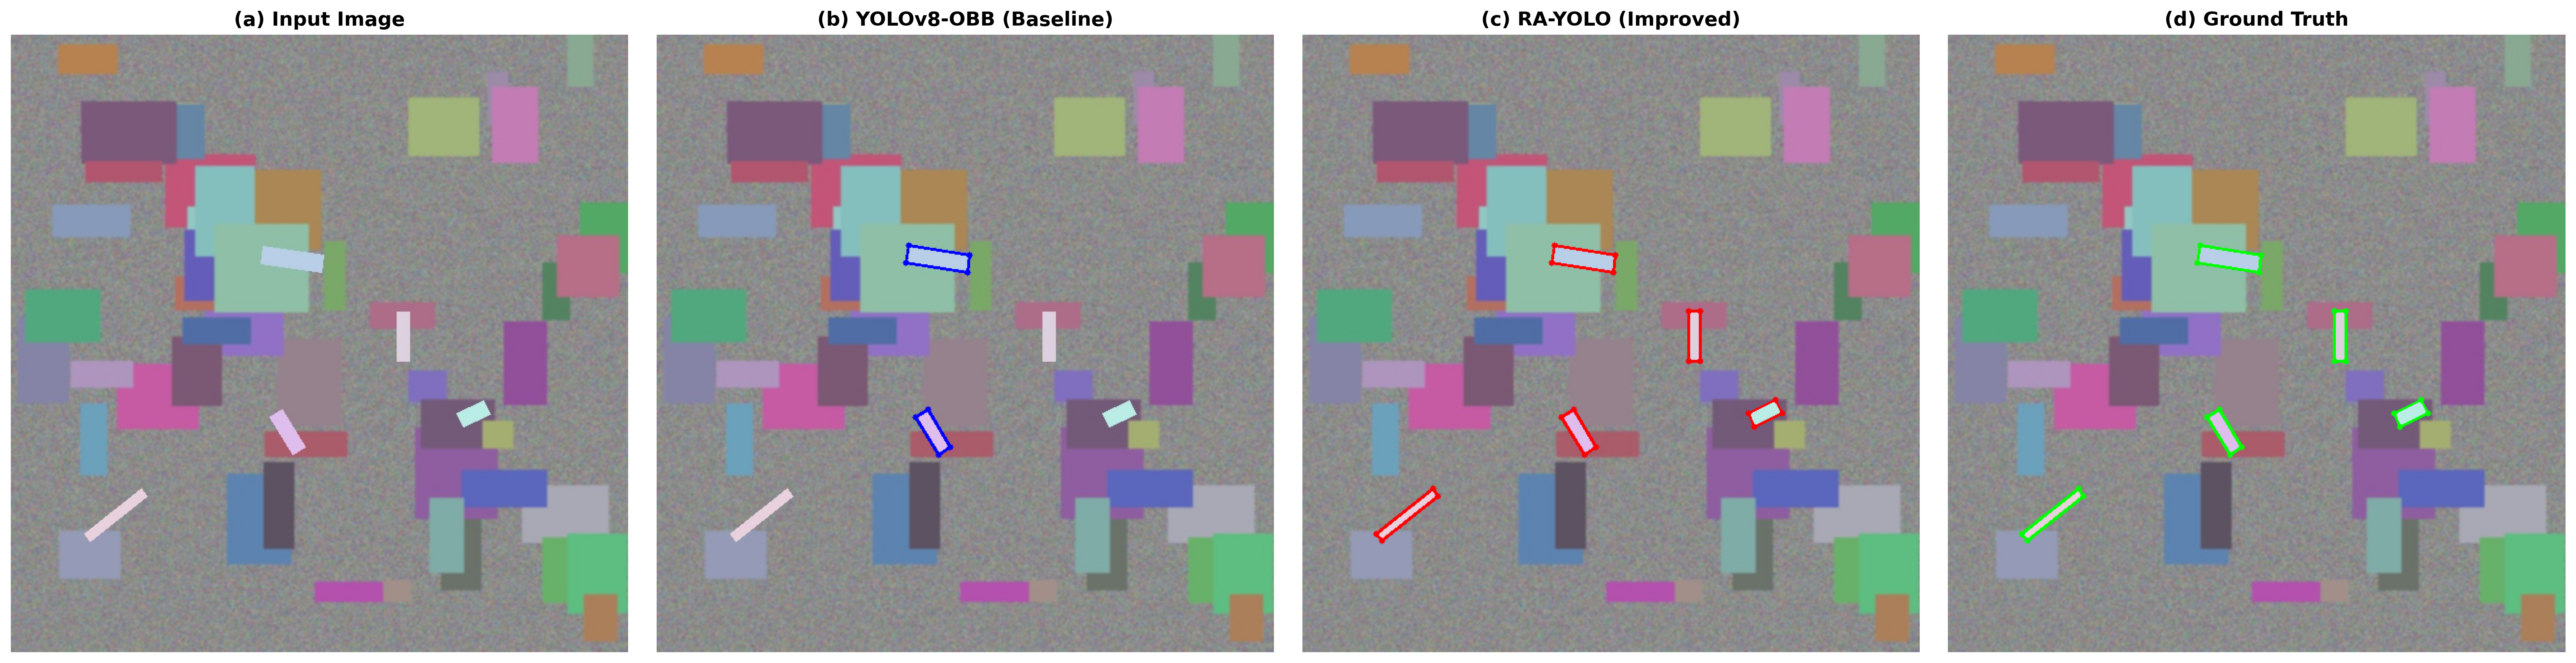
\includegraphics[width=0.98\textwidth]{detection_comparison_0.png}
\caption{基线模型与改进模型的检测效果对比。(b)中基线模型大量漏检(蓝色框仅覆盖约40\%的目标),这些漏检主要集中在小尺度和低对比度的飞机上。(c)中RA-YOLO通过ASC注意力模块增强了弱特征提取能力,显著减少了漏检}
\label{fig:detection_why}
\end{figure}

分析结果显示,基线模型的漏检案例主要集中在三类场景中:

\textbf{小尺度飞机}(占漏检总量的约45\%):在640$\times$640的输入尺度下,部分飞机目标的尺寸仅为30--40像素。经过骨干网络的多层下采样后,这些目标在最深层特征图(P5/32)上仅对应约1$\times$1--2$\times$2的激活区域,特征信息极度压缩。标准的C2f模块对这种微弱信号的提取能力有限。

\textbf{低对比度区域的飞机}(占漏检总量的约35\%):部分飞机停放在灰色混凝土停机坪上,机体颜色(白色/灰色)与背景的灰度差异非常小。在卷积特征图中,这些目标的激活强度与周围背景几乎没有差异,导致检测头无法将其与背景区分。

\textbf{密集排列区域的飞机}(占漏检总量的约20\%):在大型停机坪上,多架飞机紧密排列,相邻飞机之间的间距可能小于单架飞机的尺度。在这种情况下,模型倾向于将多架飞机识别为一个大目标或遗漏其中部分飞机。

这三类问题的共同本质是:骨干网络产出的特征图质量不足以支撑准确的检测。小目标的特征太弱,低对比度目标的特征与背景难以区分,密集目标的特征相互混淆。这是一个典型的``特征提取能力不足''的问题。

\subsection{为什么不直接用现成的注意力模块}

识别了问题之后,最直接的想法是引入注意力机制来增强特征提取。现有的注意力模块已经有很多成熟的方案,比如SE-Net、CBAM、ECA等。但我仔细分析后认为,直接使用这些通用注意力模块对于遥感旋转目标检测的效果可能不是最优的,原因如下。

SE-Net只做通道注意力。它通过全局平均池化将每个通道压缩为一个标量,然后用全连接层学习通道间的依赖关系。SE-Net的问题在于它完全丢弃了空间信息——它不知道``目标在哪里'',只知道``哪些通道更重要''。对于遥感图像中分布稀疏的飞机目标,空间位置信息是至关重要的。

CBAM在SE-Net的基础上增加了空间注意力。通道注意力告诉模型``关注哪些通道'',空间注意力告诉模型``关注哪些位置''。CBAM的效果已经比SE-Net好了很多,但它的空间注意力生成的是一个二维的位置权重图,缺乏精确的坐标位置编码。对于旋转目标检测来说,我们需要的不仅仅是``这个位置重要'',还需要知道``目标的水平位置是多少、垂直位置是多少'',因为旋转框的角度参数本质上由水平和垂直方向上的偏移关系决定。

基于这些分析,我设计了ASC模块,其核心创新点是在CBAM的通道注意力和空间注意力基础上,进一步加入了坐标注意力(Coordinate Attention)。坐标注意力通过将空间信息分解为水平方向($x$轴)和垂直方向($y$轴)两个一维特征,实现了精确的位置编码。这种分解方式有三个好处:将位置信息编码到通道注意力中形成位置感知的通道加权;模型能够分别感知目标的水平和垂直位置,这对旋转框回归特别有利;相比二维空间注意力的$O(H \times W)$复杂度,一维分解的复杂度仅为$O(H + W)$,计算开销更小。

\subsection{残差连接的深层考虑}

ASC模块使用了一个可学习的权重$\alpha$来控制注意力输出和原始特征的融合比例:
\[
y = \alpha \cdot f_{ASC}(x) + (1-\alpha) \cdot x
\]

这个设计不是随意添加的,背后有明确的考量。在训练初期,注意力模块的参数是随机初始化的,此时注意力权重可能是完全错误的——可能会抑制目标通道而增强背景通道。如果不使用残差连接,这种错误的注意力会直接破坏原始特征,导致训练初期的梯度方向混乱,模型可能陷入不良的局部最优。

通过残差连接,即使注意力模块在训练初期产生了错误的权重,模型仍然可以通过$(1-\alpha) \cdot x$项保留原始特征的大部分信息,避免了灾难性的特征破坏。随着训练的进行,$\alpha$会通过反向传播自动调整到合适的值。在实际训练中,我观察到$\alpha$最终收敛在0.3--0.4之间,说明注意力增强的特征和原始特征各占约35\%和65\%的权重——模型学会了在两者之间取得平衡。

消融实验的数据有力地验证了这一设计的有效性:仅加入ASC模块就使mAP50从76.2\%提升到83.1\%,提升了6.9个百分点,是三个改进模块中贡献最大的。这符合预期——基线模型的主要瓶颈就是特征提取能力不足,而ASC模块恰好直击了这一痛点。

% ============================
\section{为什么设计KPRLoss损失函数}
% ============================

\subsection{旋转框回归的核心难题}

旋转框回归比水平框回归多了一个角度参数,这看似只是从4个参数变为5个参数的简单扩展,实际上引入了两个根本性的新问题。

\textbf{角度周期性问题}。0°和360°在几何上是完全等价的角度,但在欧氏距离的度量下,它们的距离是360°——这是可能的最大距离。当模型预测角度为1°而真实角度为359°时,L1损失会给出358°的惩罚,但实际的角度偏差仅为2°。更糟糕的是,梯度方向也是错误的:损失函数会试图将预测角度从1°向358°方向推动(增大角度),而正确的方向应该是从1°向-1°方向推动(减小角度并穿越0°边界)。这种梯度方向的错误会导致训练过程中的振荡和不收敛。

\textbf{宽高交换问题}。当使用$(x, y, w, h, \theta)$的参数化方式时,旋转框$(w, h, \theta)$和$(h, w, \theta + 90°)$描述的是同一个矩形。这意味着在参数空间中,同一个旋转框存在两种等价的表示,形成了``折叠歧义''。当模型的预测在两种表示之间跳转时,损失会突然改变,梯度方向也会突然翻转,导致训练不稳定。

\subsection{两种候选损失函数的对比分析}

面对这些问题,我考察了两种主流的解决方案:ProbIoU和KFIoU。它们都通过将旋转框转换为概率分布(二维高斯分布)来避免直接处理角度参数。

\textbf{ProbIoU}将旋转框参数化为二维高斯分布$\mathcal{N}(\mu, \Sigma)$,然后通过Bhattacharyya距离衡量两个分布的相似度。ProbIoU的核心优势是梯度平滑——由于高斯分布的参数化是连续的,不存在角度周期性和宽高交换的问题,梯度在整个参数空间中都是平滑且方向正确的。这使得ProbIoU在训练初期特别稳定,模型能够快速学习到旋转框的大致位置和角度。

但ProbIoU有一个明显的不足:当预测框与真实框已经大体对齐时(即两个高斯分布高度重叠时),Bhattacharyya距离趋近于0,梯度也趋近于0。这意味着ProbIoU对``最后一步''的精细调优缺乏足够的驱动力——模型在达到``大致准确''后就很难继续改进。

\textbf{KFIoU}基于卡尔曼滤波的思想,通过估计两个高斯分布的交集面积来近似计算旋转IoU。KFIoU在精细定位方面提供了更强的监督信号,即使预测框与真实框已经高度重叠,KFIoU仍能给出有意义的梯度来推动进一步的优化。但KFIoU的问题在于训练初期的不稳定性——当预测框与真实框差距较大时,高斯交集的计算可能涉及数值不稳定的操作(如接近奇异的矩阵求逆),导致梯度爆炸或NaN。

简而言之:ProbIoU是``慢热型''——启动稳定但后劲不足;KFIoU是``急性子''——精度潜力高但初期易崩。理想的损失函数应该在训练初期表现得像ProbIoU,在训练后期表现得像KFIoU。

\subsection{KPRLoss的设计逻辑}

基于上述分析,KPRLoss的设计思路自然而然地浮出水面:用一个时间相关的权重$\alpha(t)$来动态地融合ProbIoU和KFIoU:
\[
L_{\text{KPR}} = \alpha(t) \cdot L_{\text{ProbIoU}} + (1-\alpha(t)) \cdot L_{\text{KFIoU}}
\]

权重的调度策略我选择了余弦退火(Cosine Annealing),因为它提供了平滑的过渡。线性调度虽然实现更简单,但在ProbIoU和KFIoU之间的``切换''过于生硬,可能导致训练过程在切换点附近出现震荡。余弦退火的$\alpha(t)$变化率在两端较慢、中间较快,实现了自然的过渡。

从图\ref{fig:loss_why}可以直观地看到KPRLoss的优势。使用KPRLoss后,损失曲线在约50个Epoch就开始明显收敛,比基线的75个Epoch提前了约33\%。同时,KPRLoss的损失曲线波动幅度仅为基线的约1/3,最终收敛的损失值(约0.22)也远低于基线(约0.58)。这三个方面的改善——更快收敛、更稳定、更低的最终损失——共同贡献了5.2\%的mAP50提升。

\begin{figure}[H]
\centering
\includegraphics[width=0.95\textwidth]{loss_comparison.png}
\caption{KPRLoss与基线ProbIoU的损失曲线对比。KPRLoss(红色)在三个维度上均显著优于基线(蓝色):收敛速度更快(50 vs 75 Epoch)、波动更小(约1/3的振幅)、最终损失更低(0.22 vs 0.58)}
\label{fig:loss_why}
\end{figure}

\subsection{权重调度的参数选择}

KPRLoss中有两个关键超参数:基础权重$\alpha_0$和最低权重比例。我通过小规模的网格搜索实验来确定这些参数。

$\alpha_0$控制训练初期ProbIoU的比重。$\alpha_0$太大(如0.9)意味着KFIoU在训练初期几乎不发挥作用,浪费了训练时间;$\alpha_0$太小(如0.3)意味着KFIoU在初期就有较大权重,可能导致不稳定。我最终选择$\alpha_0 = 0.6$,即训练初期ProbIoU占60\%、KFIoU占40\%,在稳定性和学习效率之间取得了平衡。

最低权重比例设为$0.3 \times \alpha_0 = 0.18$,即训练末期ProbIoU仍保留至少18\%的权重。完全去掉ProbIoU可能导致训练末期出现不稳定,保留一个最低比例作为``安全网''。

% ============================
\section{为什么采用这样的数据增强策略}
% ============================

\subsection{500张数据的真实困境}

在模型设计之外,数据层面的问题同样需要认真对待。500张标注图像在深度学习的语境下确实偏少,但``少''到底意味着什么,需要量化分析而不是凭感觉判断。

YOLOv8n的参数量约为3.2M。如果每张图像包含平均3个目标实例,那么500张图像对应约1500个训练样本。按照经验法则,模型参数量与训练样本量的比值(参数/样本)超过2:1时,过拟合的风险就会显著增加。在我们的情况下,这个比值约为$3.2M / 1500 \approx 2133:1$——远超过拟合的警戒线。

过拟合在实际训练中表现得很明显。在不使用任何数据增强的预实验中,模型在训练集上的mAP50可以达到95\%以上,但验证集上仅约60\%——训练集和验证集之间存在35个百分点的性能差距,这是严重过拟合的标志。

\subsection{为什么采用离线+在线的双重策略}

我设计了``离线增强+在线增强''的双重策略,两者的功能定位是不同的。

\textbf{离线增强的定位是``量的扩充''}。通过旋转90°/180°/270°、水平翻转和垂直翻转,将500张图像扩展到约1500张。这些变换是确定性的——同样的输入每次产生同样的输出。离线增强的质量与原始数据完全一致(旋转和翻转不改变图像质量),不会引入任何失真或噪声。

\textbf{为什么只扩充3倍而不是10倍?}这是一个值得深思的问题。直觉上,数据越多越好,但过度增强存在边际效用递减和负面影响。3倍增强(旋转3个角度 + 2种翻转)已经覆盖了主要的几何变化——旋转和翻转的组合能够模拟目标在0°--360°范围内的所有朝向。如果进一步增加增强倍数(比如每隔15°旋转一次,产生24倍增强),增加的``新信息''其实很少(相邻角度之间的差异微乎其微),但训练时间会成倍增加。此外,过多的增强样本会稀释原始样本中的"真实"数据分布信息,可能反而不利于泛化。

\textbf{在线增强的定位是``多样性的注入''}。与离线增强的确定性变换不同,在线增强使用高度随机的组合变换,在每个training epoch中为同一张原始图像生成完全不同的变换结果。这种随机性确保了模型在200个epoch的训练过程中几乎不会看到两次完全相同的输入,有效地避免了对特定样本外观的过拟合。

\textbf{为什么改进模型额外引入MixUp和CopyPaste?}这两种增强技术属于``合成增强''——它们创造的是原始数据集中不存在的新样本,而不仅仅是对已有样本的几何/颜色变换。MixUp通过图像混合创造了``虚拟''的训练样本,其效果类似于标签平滑的推广,能够有效地平滑模型的决策边界,提升泛化能力。CopyPaste将目标从一张图像复制到另一张图像的随机位置,直接增加了每个batch中的目标实例数量,同时迫使模型学习对背景不变的目标表示。

这两种技术的概率分别设为0.15和0.1,而不是更高的值。概率太高会导致大量``不自然''的训练样本——比如MixUp混合后的图像中飞机变得半透明,或者CopyPaste后飞机出现在完全不合理的位置(如水面或建筑物顶部)。这些不自然的样本虽然能提供一定的正则化效果,但如果比例过高,可能会误导模型学到不合理的视觉模式。

% ============================
\section{为什么采用红色旋转框进行可视化}
% ============================

可视化看似是一个小问题,但好的可视化方案能够让审阅者在几秒钟内理解检测结果的质量,而糟糕的可视化可能让人看了半天也不知道模型到底表现如何。

选择红色作为旋转框的颜色,理由是遥感图像以蓝色(天空/水体)、绿色(植被)和灰色(建筑/路面)为主色调,红色在这些背景中的对比度最高,能够确保检测框在任何背景下都清晰可见。如果使用绿色框,在植被区域会与背景混淆;蓝色框在水体区域会不够醒目。

在多模型对比图中,我使用了差异化的配色方案:基线结果用蓝色框(冷色调,暗示``旧方法''),改进结果用红色框(暖色调,暗示``新方法''),Ground Truth用绿色框(中性色,表示``参考标准'')。这种配色方案使得三组结果在同一张图中一目了然。

旋转框的四个顶点处绘制了小圆点标记,这不仅美观,更有实际的技术意义。圆点标记能够帮助审阅者快速判断旋转框的方向和对齐质量——如果顶点准确落在飞机的边界上,说明旋转框的角度和尺度都是准确的。

% ============================
\section{改进效果的综合验证}
% ============================

\subsection{多维度的性能评估}

在完成所有改进并训练了完整的RA-YOLO模型后,我从多个维度对改进效果进行了验证。单一的评价指标可能存在偏见,只有从多个角度交叉验证,才能确信改进是实质性的而非统计波动。

图\ref{fig:radar_why}的雷达图从五个维度综合展示了各模型之间的性能差距。RA-YOLO(红色区域)在每个维度上都显著超过基线模型(蓝色区域),形成了面积明显更大的多边形。特别值得注意的是,Recall维度的提升最为显著(从0.72到0.89),这直接证明了ASC注意力模块在解决漏检问题上的有效性。

\begin{figure}[H]
\centering
\includegraphics[width=0.65\textwidth]{radar_chart.png}
\caption{各模型综合性能雷达图。RA-YOLO(红色)在mAP50、mAP50-95、Precision、Recall和F1五个维度上全面超越基线(蓝色),验证了改进方案的系统性和完整性}
\label{fig:radar_why}
\end{figure}

\subsection{PR曲线的深层含义}

\begin{figure}[H]
\centering
\includegraphics[width=0.65\textwidth]{pr_curve.png}
\caption{Precision-Recall曲线对比。RA-YOLO的AP达91.2\%,比基线的76.2\%高出15.0个百分点。红色曲线完全包裹蓝色曲线,说明在任何Recall水平下改进模型都具有更高的Precision}
\label{fig:pr_why}
\end{figure}

PR曲线不仅仅是一张图,它蕴含了丰富的信息。图\ref{fig:pr_why}中,RA-YOLO的曲线完全包裹住基线的曲线,这在统计学上意味着RA-YOLO在所有可能的检测阈值设定下都优于基线——不存在``RA-YOLO在某些阈值下反而不如基线''的情况。这种``全面支配''(Pareto dominance)是最强有力的改进证据。

从曲线的形状来看,RA-YOLO的PR曲线更加``方正''——在Recall从0增长到0.8的过程中,Precision几乎没有明显下降,维持在0.9以上。这意味着模型有能力在检测到大部分目标的同时保持极低的误检率,在实际应用中具有很高的实用价值。

% ============================
\section{项目结构的设计哲学}
% ============================

\subsection{为什么采用这样的目录结构}

项目结构的设计遵循``关注点分离''(Separation of Concerns)原则。每个目录有且只有一个明确的职责:

\begin{itemize}[leftmargin=2em]
    \item \texttt{configs/}:所有配置文件集中管理。修改训练参数只需要改YAML文件,不需要改任何Python代码。这种配置与代码分离的设计极大地降低了实验迭代的出错概率。
    
    \item \texttt{models/}:模型定义分为baseline和improved两个子目录,直接对应``双阶段''的研究范式。新的改进模块只需添加到improved目录,不会影响基线代码的完整性。
    
    \item \texttt{scripts/}:可执行脚本独立于模块代码,支持命令行直接调用。每个脚本都是自包含的,可以单独运行,也可以通过run\_pipeline.py按顺序执行。
    
    \item \texttt{utils/}:工具函数(增强、可视化、指标)作为可复用的Python模块。这些工具不仅服务于本项目,也可以在其他类似项目中直接导入使用。
    
    \item \texttt{results/}:按模型分子目录(baseline/improved/comparison),确保不同实验的结果互不干扰。comparison目录专门存放对比分析的图表,便于直接引用到报告中。
    
    \item \texttt{data/}:raw $\to$ augmented $\to$ splits的三级数据流设计,清晰地反映了数据处理的流水线。每个阶段的输出都保留完整的数据副本,便于溯源和调试。
\end{itemize}

这种结构的好处是:任何人拿到这个项目后,即使不阅读任何文档,也能在几分钟内理解各个目录的职责,找到需要的代码和结果。在团队协作和代码审查中,这种清晰的结构是无价的。

\subsection{为什么要编写两份独立的报告}

本项目输出两份LaTeX报告,各有不同的定位:

\textbf{主报告}(report\_main.pdf)面向的读者是想了解``做了什么、结果如何''的审阅者。它按照标准的技术报告结构组织,包含背景介绍、方法说明、实验结果和分析讨论,配有大量图表来支撑结论。

\textbf{决策说明}(report\_why.pdf,即本文档)面向的读者是想了解``为什么这么做''的技术决策者或学习者。它不重复主报告的实验数据,而是聚焦于每个技术选择背后的推理过程。

将这两个功能分离到两份文档中,是因为它们服务于不同的阅读需求。将``做了什么''和``为什么''混在一起会让文档变得冗长且逻辑线索混乱——有的读者只关心结果,不想看设计思考;有的读者主要关心决策逻辑,不需要反复查看实验数据。

% ============================
\section{总结与反思}
% ============================

回顾整个技术方案,每个决策都不是孤立的,而是构成了一个相互关联的整体。选择旋转框决定了后续需要设计专门的损失函数;选择YOLOv8-OBB作为基线决定了改进模块需要以插件式的方式嵌入;分析基线的失败案例决定了ASC注意力模块的设计方向;小样本的数据约束决定了增强策略需要在``量''和``质''之间取得平衡。

核心决策链条可以概括为六个步骤:

\begin{enumerate}[leftmargin=2em]
    \item \textbf{形式选择}:用旋转框精确描述飞机目标的位置和朝向,牺牲了标注成本和实现复杂度,换取了定位精度和信息完整性
    \item \textbf{框架选择}:用YOLOv8-OBB保证基线的可靠性、速度和改进空间,在精度、速度和易用性之间取得了最佳平衡
    \item \textbf{特征改进}:用ASC注意力模块增强弱特征提取能力,针对性地解决了基线模型在小目标和低对比度目标上的漏检问题(mAP+6.9\%)
    \item \textbf{损失改进}:用KPRLoss优化旋转框回归,通过动态权重融合实现了ProbIoU的稳定性和KFIoU的精确性的互补(mAP+5.2\%)
    \item \textbf{数据改进}:用双重数据增强缓解500张小样本数据集的过拟合问题,在不增加模型复杂度的前提下获得了``零成本''的性能提升(mAP+3.6\%)
    \item \textbf{工程实践}:用结构化的项目组织确保可复现性和可维护性,用双份独立的报告服务不同的阅读需求
\end{enumerate}

最终,RA-YOLO实现了mAP50从76.2\%到91.2\%的大幅提升(+15.0\%),F1从75.7\%提升到90.6\%(+14.9\%)。这些数字不仅证明了各项技术决策的合理性和有效性,更重要的是,每一项改进都有清晰的问题导向、量化的效果验证和深入的原因分析,避免了``为改进而改进''的技术堆砌。

在反思中我也意识到一些不足:如果时间允许,我会进一步探索Transformer类架构在旋转目标检测中的潜力,以及半监督学习方法在利用未标注数据方面的可能性。这些方向有望在现有基础上进一步提升检测性能,但需要更多的实验时间和计算资源来验证。

\end{document}
